% --------------------------------------------------------------------------
% Version 2.1
% This template is available on the sites:
% https://www.overleaf.com/read/rpkkfchcnbsc
% https://www.overleaf.com/latex/templates/itmo-beamer-theme/fpttrgnmqwsb
% https://github.com/AlexZabashta/ITMO-Beamer-theme
% --------------------------------------------------------------------------

% Attention!!!
% This document was created only as an example of using ITMO beamer styling.
% Don't use it as a Latex or beamer tutorial!
% Check out the capabilities of Latex and beamer (at least basic) independently.


\documentclass[aspectratio=169]{beamer}
\usepackage{ITMOtheme}


% Use this package to automatically format references.
% \usepackage[style=mla]{biblatex}
% \addbibresource{references.bib}


\titlegraphic{
\includegraphics[scale=0.2]{itmo/logo_en_vert_blue.pdf}}

% The fields 'title', 'author', 'subject', 'keywords' are used to generate a PDF document.
% It is recommended that you fill them in, even if you are creating your title slide manually.

% use \title[short title]{full title}
\title[Simplificación Funciones Lógicas]{Simplificación Funciones Lógicas}

%\subtitle[short subtitle]{long subtitle}

\author[Rodríguez J.]{Juan Felipe Rodríguez Galindo}

%\institute[short institute]{long institute}

\where{Bogotá D.C.}
\date{\today}


\subject{Simplificación de funciones lógicas}
\keywords{Universidad Distrital, Arquitectura, Funciones Lógicas}


% By default, the title of the presentation (\inserttitle) is written at the bottom of each slide.
% This text can be replaced with something else, for example:
\setfootlinetext{\insertsection}


\begin{document}


% [plain] - modifier to create a blank slide (without bottom bar).
% Ideal for creating the first (title) and last slide with a polygonal background,
% or for transitional slides between chapters or slides with a table of contents.

% \titlepage - command for automatic generation of title slide content.

\begin{frame}[plain]
    \titlepage
\end{frame}

% You can use custom title, if you want.
% Or you can you modify the .sty file.


\begin{frame}[plain]
	\itmopolygons{
	\vfill
		
\includegraphics[scale=.2]{itmo/logo_en_vert_blue.pdf}
	\vfill
		\usebeamerfont{title}{  \inserttitle\par} 
	\vfill
		\insertauthor\par
	\vfill
	    Código 20181020158
	\vfill
		\insertplace  \;  \insertdate
}
\end{frame}


% Avoid making a table of contents in short presentations.
% Transitions between chapters are best done manually.

\AtBeginSection[]
{
    \begin{frame}[plain]
        \frametitle{Indice}
        %\Large
        \tableofcontents[currentsection]
    \end{frame}
}

\section{Introducción} 

\begin{frame}{Resumen}

En el presente documento se enunciará como a través de la aplicación del álgebra booleana y los mapas de \textit{Karnaugh}, principalmente pasaremos de una revisión del marco teórico, explicación básica de su funcionamiento a través de ejercicios y las respectivas conclusiones de la temática tratada.
% \footnote{For example, it can be used for citation.}

\end{frame}


\begin{frame}
\frametitle{Introducción}

E{\MakeLowercase{ste}} artículo presenta el uso, aplicación y manejo del álgebra lineal o los mapas de \textit{Karnaugh}. Se fundamenta en explicar al lector el conocimiento básico en cuanto a simplificación de funciones lógicas y el cómo se pueden aplicar estos conocimientos.\\
\hspace{2px} \\
La \alert{aplicación de métodos de simplificación de álgebra booleana y mapas de \textit{Karnaugh}}; en las circunstancias correctas permiten al desarrollador implementar dentro del circuito o la ecuación la solución óptima y la mejor calidad de  producto final, por esto el buen entendimiento de estos métodos es fundamental en la aplicación de la simplificación de funciones lógicas.\\

\end{frame}

\begin{frame}
\frametitle{Introducción}

El documento se dividirá en \alert{tres grandes etapas o secciones, en la primera} se le dará una introducción a que es una simplificación de funciones, \alert{anexo a la sección anterior} se verán algunos de los tipos más reconocidos de simplificación, es decir por medio de la aplicación de álgebra booleana y mapas de \textit{Karnaugh}. \alert{Por último} se revisará su aplicación, y la conclusión del tema observado junto con la percepción del autor sobre la temática.

\end{frame}

\section{Conceptos previos}

\subsection{Circuitos, tipos y funciones lógicas}

\begin{frame}
\frametitle{Circuitos y tipos}

\begin{block}{Circuitos digitales}
Se considera circuito digital a \alert{todo aquel circuito que maneje toda la información que maneja de forma binaria}, estos tienen a su vez una serie de componentes necesarios para su funcionamiento, tanto \alert{circuitos electrónicos activos y pasivos}, conectado entre el ingreso de energía y tierra.
\end{block}

\end{frame}

\begin{frame}
\frametitle{Circuitos y tipos}
\begin{block}{Tipos de circuitos}
Existen dos tipos principales de circuitos:
\end{block}

\begin{exampleblock}{Circuito secuencial}
El secuencial que es aquel que depende de las entradas anteriores y las actuales de igual forma, podemos definirla como un circuito que posee memoria.
\end{exampleblock}

\begin{alertblock}{Circuito combinacional}
El combinacional el cual es el que vamos a manejar es aquel que depende solamente de la entrada en el instante.
\end{alertblock}
\end{frame}

\begin{frame}
\frametitle{Funciones Lógica}
\begin{block}{Funciones Lógicas}
Para especificar el funcionamiento de un circuito debemos tener en cuenta el concepto de Función Lógica, el cual se puede definir como  \alert{"la representación formal de un circuito digital"}\footnote{tomado de \href{https://cutt.ly/Funciones_Logicas}{Martí Campoy, A. (2018). Funciones lógicas: tabla de verdad.}}. En su mayoría se destaca el uso dentro de los circuitos digitales combinacionales.
\end{block}
\end{frame}

\begin{frame}
\frametitle{Funciones Lógica}
\begin{block}{Notas importantes funciones lógicas}
Hay que tener en cuenta dentro de la definición de función lógica, a la que \alert{esta se refiere a cualquier forma de representar o expresar el funcionamiento que queremos que tenga un circuito}.\\
\hspace{2px}
\\En segundo lugar, tenemos que tener en cuenta que este es de tipo formal, \alert{lo cual quiere decir que tiene que haber unas reglas que nos guíen al momento de representar estos comportamientos}.
\end{block}
\end{frame}

\section{Marco teórico}

\subsection{Álgebra de booleana y diagramas de \textit{Karnaugh}}

\begin{frame}
\frametitle{Álgebra de Bool}

\textcolor{ITMOtomato}{Sistema algebraico} formado por un conjunto \textcolor{ITMOtomato}{B}=\{\textcolor{ITMOtomato}{0},\textcolor{ITMOtomato}{a},\textcolor{ITMOtomato}{b}, ... ,\textcolor{ITMOtomato}{1}\} finito, y que tiene o cumple con dos operaciones [\textcolor{ITMOtomato}{\(+\)},\textcolor{ITMOtomato}{\(\cdot\)}], que cumplen con los postulados para cualesquiera elementos \textcolor{ITMOtomato}{X}, \textcolor{ITMOtomato}{Y}, \textcolor{ITMOtomato}{\(Z \in B\)}:\\

\centering{
    Propiedad de pertenencia\\
    \Rightarrow \textcolor{ITMOorange}{ \(X+Y \in B\)},\textcolor{ITMOorange}{\( X \cdot Y \in B\)}\\
    
    Propiedad conmutativa\\ 
    \Rightarrow \textcolor{ITMOorange}{ X+Y }=\textcolor{ITMOorange}{ Y+X }; \textcolor{ITMOorange}{ \(X \cdot Y\) }=\textcolor{ITMOorange}{ \(Y \cdot X\) }\\
    
    Propiedad distributiva\\ 
    
    \Rightarrow
    \textcolor{ITMOorange}{ \(X \cdot (Y+Z)\) }=\textcolor{ITMOorange}{  \( (X \cdot Y)\) + \( (X \cdot Z)\) };\\
    \textcolor{ITMOorange}{ X \cdot \(Y+Z\) }=\textcolor{ITMOorange}{ \( (X+Y) \cdot (X+Z)\) }\\
    
    Elemento identidad\\ 
    \Rightarrow 
    \textcolor{ITMOorange}{X+0}=\textcolor{ITMOorange}{X}; 
    \textcolor{ITMOorange}{ \(X \cdot 1\) }=\textcolor{ITMOorange}{1}\\
    
    Elemento complementado\\ 
    \Rightarrow
    Para \textcolor{ITMOgreen}{X} existe \textcolor{ITMOgreen}{\(X \in B\)}, tal que 
    \textcolor{ITMOorange}{X+0}=\textcolor{ITMOorange}{X}; \textcolor{ITMOorange}{ \(X \cdot 1\) }=\textcolor{ITMOorange}{1}\\
}

\end{frame}

\begin{frame}
\frametitle{Álgebra de Conmutación}

Ahora observaremos el procedimiento para el sistema algebraico formado por el conjunto A = \{0,1\}, con las siguientes operaciones [\textcolor{ITMOtomato}{\(+\)},\textcolor{ITMOtomato}{\(\cdot\)}].\\
\hspace{2px}\\
\begin{columns}[c]

\column{.45\textwidth}{
    \begin{tabular}{|r r | r|} 
        $X \times$ & $Y$ & $X + Y$ \\ \hline
        $0$ & $0$ & $0$ \\
        $0$ & $1$ & $1$ \\
        $1$ & $0$ & $1$ \\
        $1$ & $1$ & $1$ \\
    \end{tabular}   
}

\column{.45\textwidth}{
    \begin{tabular}{|r r | r|} 
        $X +$ & $Y$ & $X \times Y$ \\ \hline
        $0$ & $0$ & $0$ \\
        $0$ & $1$ & $0$ \\
        $1$ & $0$ & $0$ \\
        $1$ & $1$ & $1$ \\
    \end{tabular}   
}

\column{.45\textwidth}{
    \begin{tabular}{| r | r |} 
        $X$ & $X'$ \\ \hline
        $0$ & $1$ \\
        $1$ & $0$ \\
    \end{tabular}   
}

\end{columns}
\hspace{2px}\\
Respetando así también los postulados de Boole.
\end{frame}

\begin{frame}
\frametitle{Teoremas del álgebra de Bool}

Estos teoremas se demuestran a partir de los postulados del álgebra de Boole y se aplican a cualquier álgebra de Boole, incluido el álgebra de conmutación.
La aplicación de estos teoremas permite la modificación o la simplificación de expresiones lógicas por otras equivalentes.

\centering{
    Principio de dualidad\\
    \textcolor{ITMOorange}{ \(X+1=1 \)},\textcolor{ITMOorange}{\( X \cdot Y = 0\)}\\
    
}

\end{frame}

\begin{frame}{Teoremas de boole}
    \begin{figure}
        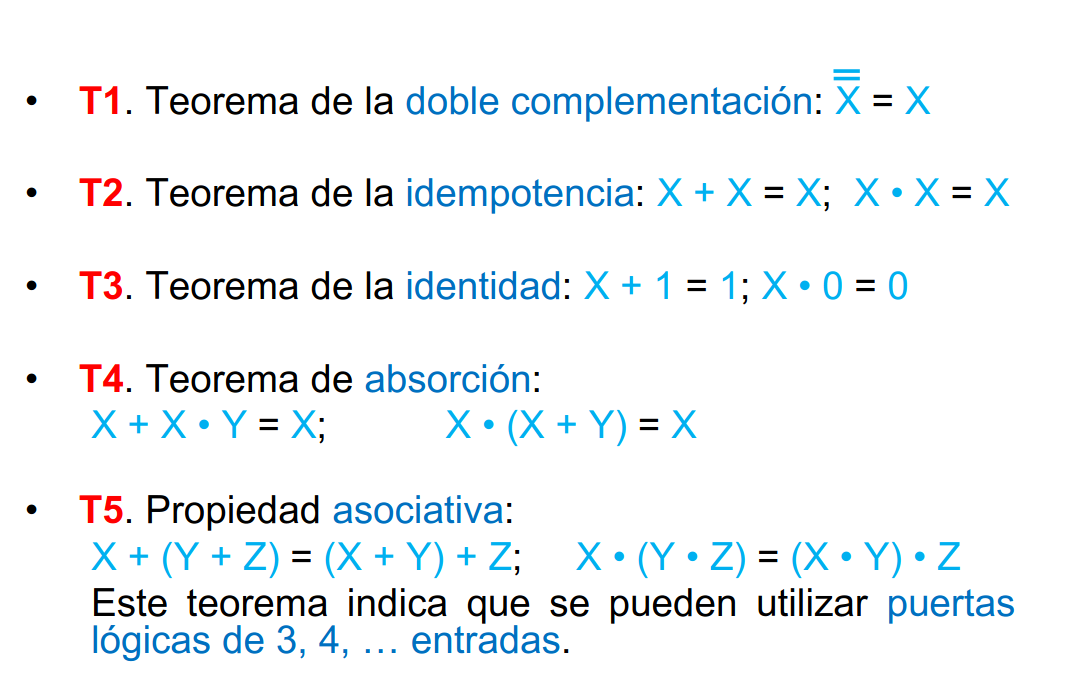
\includegraphics[scale=.3]{fig/prop_1.png}
    \end{figure}
\end{frame}

\begin{frame}{Teoremas de boole}
    \begin{figure}
        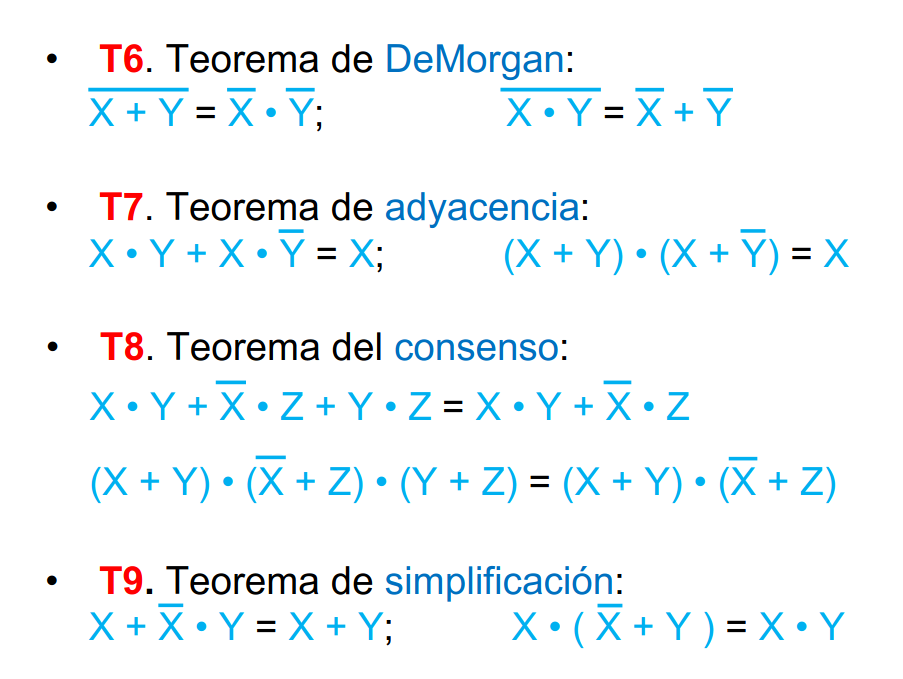
\includegraphics[scale=.3]{fig/prop_2.png}
    \end{figure}
\end{frame}

\begin{frame}
\frametitle{Simplificación de Funciones Lógica}
    \alert{Una expresión booleana o especificación lógica puede representarse de diversas maneras, sustituyendo, cambiando o re-expresando las funciones dadas por el problema original}.\\
    \hspace{2px}
    \\Las funciones lógicas nos pueden llevar a optimizar la mayoría de problemas o circuitos lógicos, llegando a tener el menor número de operaciones y términos posibles.\\
    \hspace{2px}
    \\\alert{Los teoremas y postulados nos enseñan algunas ejemplificaciones de la reducción de los circuitos digitales}.
\end{frame}

\begin{frame}{Simplificación de funciones lógicas}
    \begin{figure}
        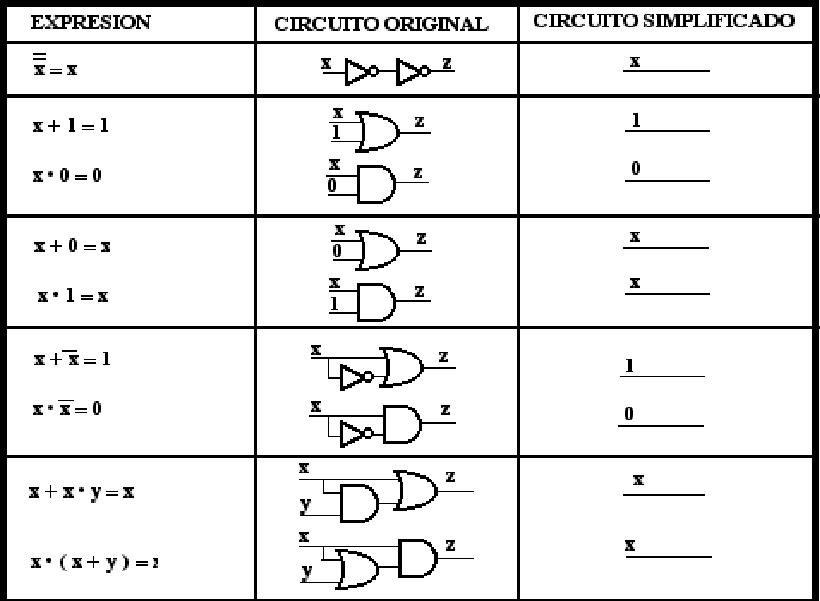
\includegraphics[scale=.3]{fig/cir_1.png}
    \end{figure}
\end{frame}

\begin{frame}{Simplificación de funciones lógicas}
    \begin{figure}
        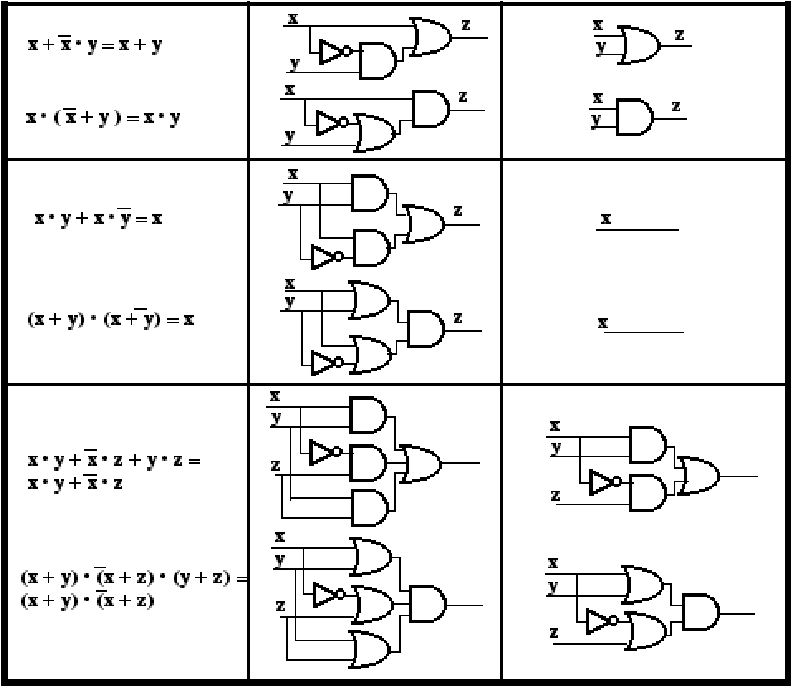
\includegraphics[scale=.28]{fig/cir_2.png}
    \end{figure}
\end{frame}

\begin{frame}{Simplificación Reglas}
    \begin{figure}
        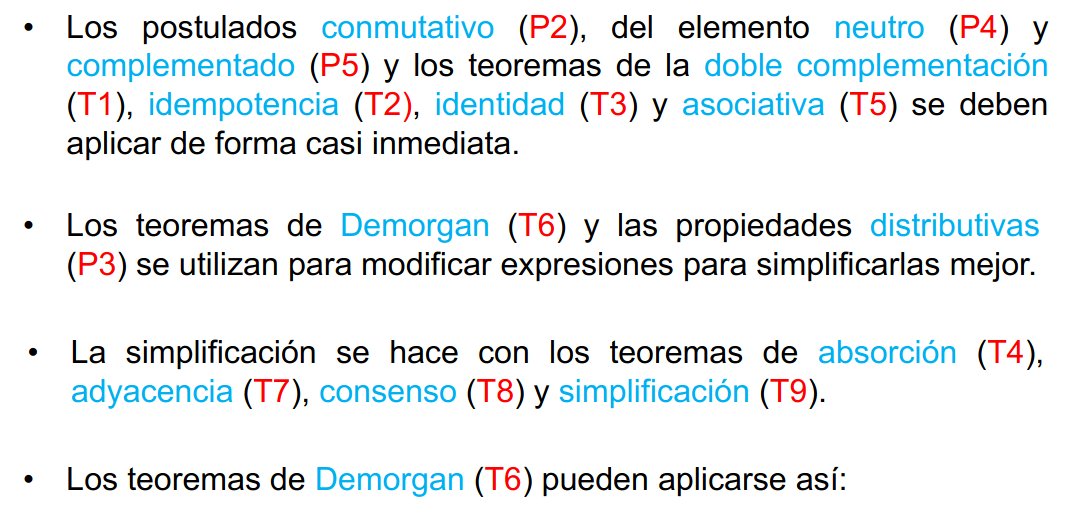
\includegraphics[scale=.28]{fig/reg_1.png}
    \end{figure}
\end{frame}

\begin{frame}{Simplificación Reglas2}
    \begin{figure}
        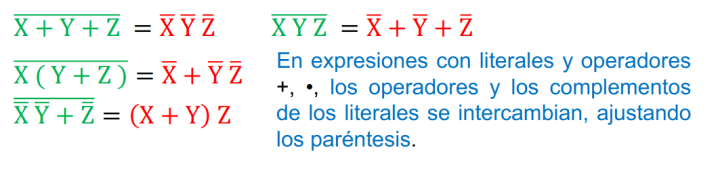
\includegraphics[scale=.4]{fig/reg_2.png}
    \end{figure}
\end{frame}

\begin{frame}
\frametitle{Diagrmas de Karnaugh}

Método gráfico que se utiliza para simplificar circuitos lógicos de forma sencilla y clara u ordenada. Este método tiene sus cimientos en todos los diferentes teoremas vistos anteriormente, su utilidad se limita a reducir 5 variables. Para este método debemos seguir las siguientes reglas:

\begin{itemize}
    \item Con base en la tabla de verdad extraer las expresiones booleana en forma de minterminos o maxterminos.
    \item Se deben asignar los "1" correspondientes en el diagrama por cada grupo de variables operadas por AND si es en forma de minterminos u operadas por OR si es en forma de maxteminos.
    \item Agrupar los "1" adyacentes (Las agrupaciones se realizan en grupos de 2,4,8 1)
    \item Eliminar las variables que aparezcan con su complemento.
    \item enlazamos con AND si es en forma de minterminos o con OR si es en forma de maxteminos
\end{itemize}
    
\end{frame}

\begin{frame}
\frametitle{Álgebra de Conmutación}

Ahora observaremos el procedimiento para el sistema algebraico formado por el conjunto A = \{0,1\}, con las siguientes operaciones [\textcolor{ITMOtomato}{\(+\)},\textcolor{ITMOtomato}{\(\cdot\)}].\\
\hspace{2px}\\

\begin{tabular}{|r r | r| r|} 
    $A$ & $B$ & $Q$ & \\ \hline
    $0$ & $0$ & $0$ & \\
    $0$ & $1$ & $0$ & $Q=(A'\cdot B)$\\
    $1$ & $0$ & $0$ & $Q=(A\cdot B')$\\
    $1$ & $1$ & $1$ & $Q=(A\cdot B)$\\
    $Q=(A'\cdot B)+(A\cdot B')+(A\cdot B)$
\end{tabular}   

\hspace{2px}
\\Ahora colocamos cada uno en el diagrama por cada grupo de variables que son operadas con AND (para nuestro ejemplo). Los diagramas de Karnaugh se presentan de forma americana o alemana.
\end{frame}

\begin{frame}{Simplificación }
    \begin{figure}
        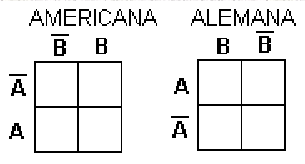
\includegraphics[scale=.4]{fig/kar_1.png}
    \end{figure}
    Podemos observar como se representa con cada una de las alternativas que tenemos, para continuar con nuestro desarrollo colocamos los 1 por cada grupo de variables operadas.\\
    \centering{
        \begin{tabular}{r | r r} 
            & $A$ & $A'$ \\ \hline
            $B$  & $0$ & $1$  \\
            $B'$ & $1$ & $1$
        \end{tabular}   
    }
    \\Ahora agrupamos los 1 adyacentes que estén al interior del diagrama, estas se realizan en grupos de 2,4,8 "1". Realizar las agrupaciones mínimas posibles.
\end{frame}

\begin{frame}{Simplificación }
    \centering{
        \begin{tabular}{r | r r} 
              & $A$ & $A'$ \\ \hline
            $B$  & $0$ & \textcolor{ITMOred}{$1$}  \\
            $B'$ & \textcolor{ITMOred}{$1$} & \textcolor{ITMOred}{$1$}
        \end{tabular}
    }
    
    Luego de realizar el agrupamiento que podemos ver con los números en rojo, eliminamos las que aparezcan con el complemento. El agrupamiento 2 "1" se elimina una variable; en el 4 "1" se eliminan 2 y en el 8 "1" se eliminan 3 variables.
    
    \begin{figure}
        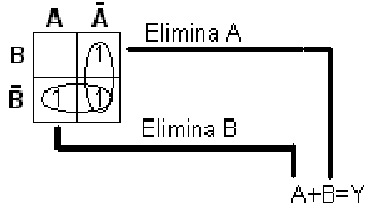
\includegraphics[scale=.4]{fig/kar_2.png}
    \end{figure}
\end{frame}

\begin{frame}{Simplificación }
    Para finalizar realizamos la operación de estos términos con OR principalmente porque estamos utilizando minterminos, teniendo en cuenta para estos los resultados que obtuvimos de la eliminación de variables.\\
    \hspace{2px}\\
    \centering{$Q=A+B$}\\
    \hspace{2px}\\
    De esta manera logramos reducir la ecuación lógica inicial a una puerta lógica OR. 
    
    
\end{frame}

%  Fin sección uno

\section{Ejemplos y aplicaciones}

\subsection{Ejemplos y aplicaciones}

\begin{frame}{Simplificación álgebra booleana}
    Ejemplo:
    
    Tenemos la ecuación (C'+D)(C+D), tenemos como fin simplificarla.\\
    (C'+D)(C+D)\\
    C'*C+C'D+DC+DD $\Rightarrow Ley distributiva$\\
    0+C'D+DC+D\\
    C'D+DC+D\\
    D(1)+D\\
    D+D\\
    $D \Rightarrow Respuesta$
    
\end{frame}

\begin{frame}{Simplificación álgebra booleana}
    Ejemplo:
    
    Tenemos la ecuación AB'D+AB'D', tenemos como fin simplificarla.\\
    AB'D+AB'D'\\
    AB'(D+D')  $\Rightarrow factorizar$\\
    AB'(1)\\
    $AB' \Rightarrow Respuesta$
    
\end{frame}

\begin{frame}{Simplificación álgebra booleana}
    Ejemplo:
    
    Tenemos la ecuación AB+A(BC)+B(B+C), tenemos como fin simplificarla.\\
    AB+AB+AC+BB+BC $\Rightarrow distributiva$\\
    AB+AB+AC+B+BC  $\Rightarrow B*B=B$\\
    AB+AC+B+BC $\Rightarrow AB+AB=AB$\\
    \textcolor{ITMOblue}{AB}+AC+\textcolor{ITMOblue}{B}+BC $\Rightarrow YX+X=X$\\
    \textcolor{ITMOblue}{B}+AC+\textcolor{ITMOblue}{BC} $\Rightarrow YX+X=X$\\
    $B+AC \Rightarrow Respuesta$
    
\end{frame}

\begin{frame}{Simplificación álgebra booleana}
    Ejemplo:
    
    Tenemos la ecuación A'BC+AB'C'+A'B'C'+AB'C+ABC, tenemos como fin simplificarla.\\
    BC(A'+A)+AB'(C'+C)+A'B'C'\\
    BC(1)+AB'(1)+A'B'C'\\
    BC+B'(A+A'C')\\
    $BC+B'A+B'C' \Rightarrow Respuesta$
    
\end{frame}
\begin{frame}{Simplificación Karnaugh}
    F(x, y, z) = x’ y’ z’ + x’ y’ z + x’ y z’+ x y’ z’+ x y z’

    \begin{tabular}{|
    >{\columncolor[HTML]{FFFFFF}}l |
    >{\columncolor[HTML]{FFFFFF}}l |
    >{\columncolor[HTML]{FFFFFF}}l |
    >{\columncolor[HTML]{FFFFFF}}l |}
    \hline
    \textbf{X} & \textbf{Y} & \textbf{Z} & \textbf{Resultado} \\ \hline
    0          & 0          & 0          & 1                  \\ \hline
    0          & 0          & 1          & 1                  \\ \hline
    0          & 1          & 0          & 1                  \\ \hline
    0          & 1          & 1          & 0                  \\ \hline
    1          & 0          & 0          & 1                  \\ \hline
    1          & 0          & 1          & 0                  \\ \hline
    1          & 1          & 0          & 1                  \\ \hline
    1          & 1          & 1          & 0                  \\ \hline
    \end{tabular}
    \begin{tabular}{lllll}
                           & 00                     & 01                     & 11                     & 10                     \\ \cline{2-5} 
    \multicolumn{1}{l|}{0} & \multicolumn{1}{l|}{1} & \multicolumn{1}{l|}{1} & \multicolumn{1}{l|}{0} & \multicolumn{1}{l|}{1} \\ \cline{2-5} 
    \multicolumn{1}{l|}{1} & \multicolumn{1}{l|}{1} & \multicolumn{1}{l|}{0} & \multicolumn{1}{l|}{0} & \multicolumn{1}{l|}{1} \\ \cline{2-5} 
    \end{tabular}\\
    
    Seguimos la teroria primero pasamos a la tabla de verdad y ya después evaluamos en el diagrama de Karnaugh.
    
\end{frame}

\begin{frame}{Simplificación Reglas}
    \begin{figure}
        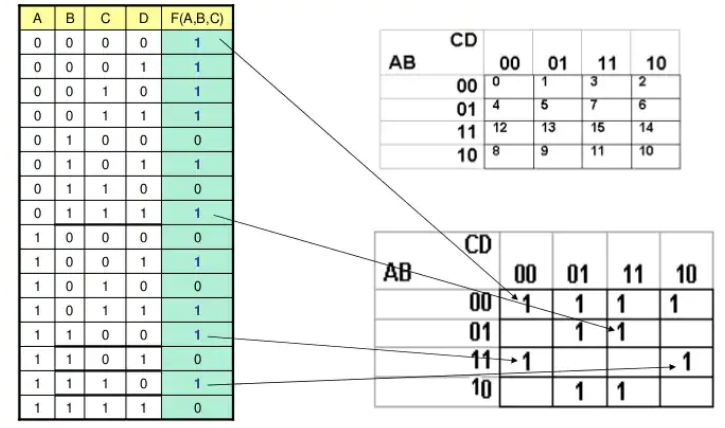
\includegraphics[scale=.5]{ejem/kar/Ejemplo.png}\footnote{Ejemplo tomado de https://es.slideshare.net/faurbano/clase06-5335816}
    \end{figure}
\end{frame}

\begin{frame}{Simplificación Reglas}
    \begin{figure}
        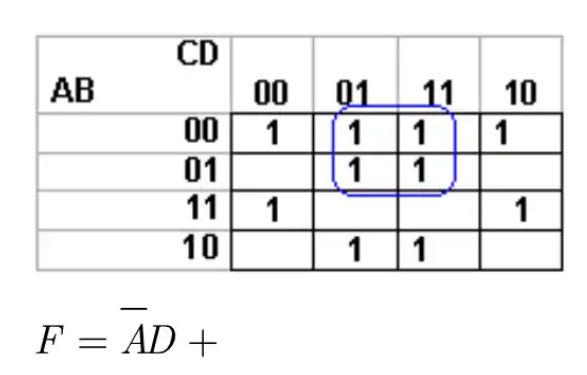
\includegraphics[scale=.4]{ejem/kar/ej_2.png}\footnote{Ejemplo tomado de https://es.slideshare.net/faurbano/clase06-5335816}
    \end{figure}
\end{frame}

\begin{frame}{Simplificación Reglas}
    \begin{figure}
        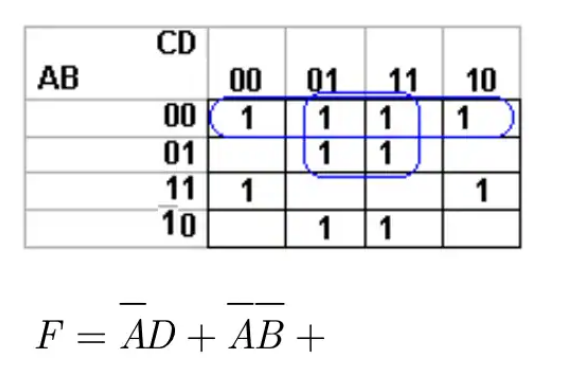
\includegraphics[scale=.4]{ejem/kar/ej_3.png}\footnote{Ejemplo tomado de https://es.slideshare.net/faurbano/clase06-5335816}
    \end{figure}
\end{frame}

\begin{frame}{Simplificación Reglas}
    \begin{figure}
        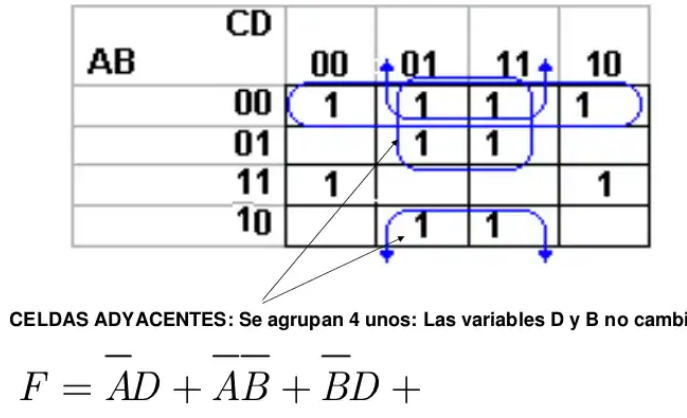
\includegraphics[scale=.4]{ejem/kar/ej_4.png}\footnote{Ejemplo tomado de https://es.slideshare.net/faurbano/clase06-5335816}
    \end{figure}
\end{frame}

\begin{frame}{Simplificación Reglas}
    \begin{figure}
        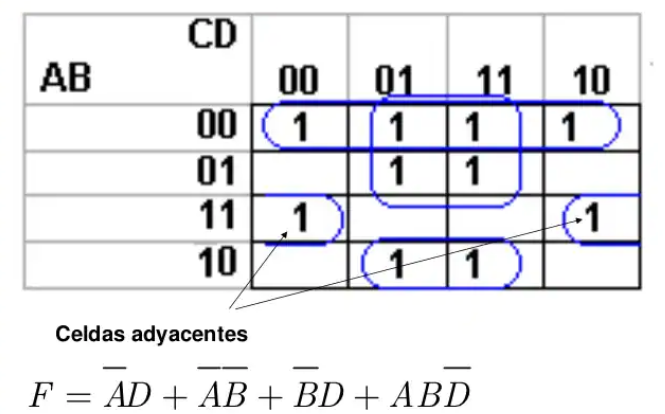
\includegraphics[scale=.4]{ejem/kar/ej_5.png}\footnote{Ejemplo tomado de https://es.slideshare.net/faurbano/clase06-5335816}
    \end{figure}
\end{frame}

\begin{frame}
\frametitle{Aplicaciones}
    Durante el proceso de estudio de la reducción y simplificación de las funciones lógicas, bajo la aplicación de álgebra booleana y diagramas karnaugh, logramos observar su aplicación directa en la tecnología actual, con el uso y aplicación de compuertas lógicas capaces de dar un a salida esperada a un circuito realizado.\\ Pudimos ver también que algunas de las propiedades arraigadas al álgebra de Bool pueden ser aplicadas al manejo o estudio de predicados, con el fin de evaluar la veracidad de una oración o discurso.\\ También sintetizar la aplicabilidad al manejo y optimización de costos para la realización de componentes electrónicos.  
\end{frame}

\section{Conclusiones y referencias}

\subsection{Conclusiones, bibliografía}


\begin{frame}
\frametitle{Conclusión}
El uso y aplicación de la simplificación de funciones lógicas es una sección fundamental del mundo moderno, así pues que con lo practicado durante la realización de este escrito nos permitió conocer a fondo como funciona para entender la lógica y los procesos que ocurren en los circuitos y aparatos electrónicos de hoy en día.\\
También nos ayuda a concebir la idea de que la optimización de cualquier sistema, llega a ser posible desde un circuito básico hasta una computadora de última generación.
\end{frame}


\begin{frame}
\frametitle{Bibliografía}
\begin{itemize}
    \item Martí Campoy, A. (2012). Generación de funciones lógicas mediante multiplexores.
    \item Acha Alegre, S., Pérez Martínez, J., Castro Gil, M. A., \& Rioseras, M. A. (2002). Electrónica Digital. Ra-Ma.
    \item Pérez, E. M., Mandado, E., \& Mandado, Y. (2007). Sistemas electrónicos digitales. Marcombo.
    \item Floyd, T. L. (1997). www. FreeLibros. org.
    \item García Merayo, F. (2015). Matemática discreta. Ediciones Paraninfo, SA.
    \item Mano, M. M. (1982). Lógica digital y diseño de computadores. Pearson Educación.
\end{itemize}
\end{frame}

\begin{frame}
\frametitle{Aprender más...}
RECURSOS BIBLIOGRÁFICOS
\begin{itemize}
    \item  \href {https://youtu.be/YgaWUWTmQnU}{ Video explicativo álgebra booleana. }   
    \item \href{https://es.slideshare.net/faurbano/clase06-5335816}{ Presentación Karnaugh}
    \item \href{https://www.youtube.com/watch?v=IYz_pKuxrZo&list=PL0_FimzlChzJPSoqfx7-RZs5wK__npj9G}{Clases Compuertas lógicas y circuitos digitales}
    \item \href{https://github.com/zhcHoward/Kmap}{Programa que realiza el mapa de Karnaugh para encontrar la simplificación de una expresión de álgebra booleana}
    \item \href{https://github.com/PyLamGR/Logic-Design-Tools}{Compendio de programas para el diseño lógico de circuitos}
    
\end{itemize}
APRENDER JUGANDO
\begin{itemize}
    \item \href{http://elibrary.matf.bg.ac.rs/bitstream/handle/123456789/297/phdBorisSobot.pdf?sequence=1}{Juegos con álgebra boolena}
    \item \href{}{}
\end{itemize}
\end{frame}


\begin{frame}[plain]
    \itmopolygons{
        \vfill
        \Huge{Fin!}
        \vfill
        
\includegraphics[scale=.2]{itmo/slogan.pdf}
    }
\end{frame}

\end{document}

% Algebra booleana
% https://youtu.be/YgaWUWTmQnU
% Karnaugh
% https://es.slideshare.net/faurbano/clase06-5335816